\documentclass[]{article}
\usepackage{lmodern}
\usepackage{amssymb,amsmath}
\usepackage{ifxetex,ifluatex}
\usepackage{fixltx2e} % provides \textsubscript
\ifnum 0\ifxetex 1\fi\ifluatex 1\fi=0 % if pdftex
  \usepackage[T1]{fontenc}
  \usepackage[utf8]{inputenc}
\else % if luatex or xelatex
  \ifxetex
    \usepackage{mathspec}
  \else
    \usepackage{fontspec}
  \fi
  \defaultfontfeatures{Ligatures=TeX,Scale=MatchLowercase}
\fi
% use upquote if available, for straight quotes in verbatim environments
\IfFileExists{upquote.sty}{\usepackage{upquote}}{}
% use microtype if available
\IfFileExists{microtype.sty}{%
\usepackage{microtype}
\UseMicrotypeSet[protrusion]{basicmath} % disable protrusion for tt fonts
}{}
\usepackage[margin=1in]{geometry}
\usepackage{hyperref}
\hypersetup{unicode=true,
            pdftitle={ADMM to solve dense submtarix problem},
            pdfauthor={Brendan Ames, Polina Bombina},
            pdfborder={0 0 0},
            breaklinks=true}
\urlstyle{same}  % don't use monospace font for urls
\usepackage{graphicx,grffile}
\makeatletter
\def\maxwidth{\ifdim\Gin@nat@width>\linewidth\linewidth\else\Gin@nat@width\fi}
\def\maxheight{\ifdim\Gin@nat@height>\textheight\textheight\else\Gin@nat@height\fi}
\makeatother
% Scale images if necessary, so that they will not overflow the page
% margins by default, and it is still possible to overwrite the defaults
% using explicit options in \includegraphics[width, height, ...]{}
\setkeys{Gin}{width=\maxwidth,height=\maxheight,keepaspectratio}
\IfFileExists{parskip.sty}{%
\usepackage{parskip}
}{% else
\setlength{\parindent}{0pt}
\setlength{\parskip}{6pt plus 2pt minus 1pt}
}
\setlength{\emergencystretch}{3em}  % prevent overfull lines
\providecommand{\tightlist}{%
  \setlength{\itemsep}{0pt}\setlength{\parskip}{0pt}}
\setcounter{secnumdepth}{0}
% Redefines (sub)paragraphs to behave more like sections
\ifx\paragraph\undefined\else
\let\oldparagraph\paragraph
\renewcommand{\paragraph}[1]{\oldparagraph{#1}\mbox{}}
\fi
\ifx\subparagraph\undefined\else
\let\oldsubparagraph\subparagraph
\renewcommand{\subparagraph}[1]{\oldsubparagraph{#1}\mbox{}}
\fi

%%% Use protect on footnotes to avoid problems with footnotes in titles
\let\rmarkdownfootnote\footnote%
\def\footnote{\protect\rmarkdownfootnote}

%%% Change title format to be more compact
\usepackage{titling}

% Create subtitle command for use in maketitle
\newcommand{\subtitle}[1]{
  \posttitle{
    \begin{center}\large#1\end{center}
    }
}

\setlength{\droptitle}{-2em}

  \title{ADMM to solve dense submtarix problem}
    \pretitle{\vspace{\droptitle}\centering\huge}
  \posttitle{\par}
    \author{Brendan Ames, Polina Bombina}
    \preauthor{\centering\large\emph}
  \postauthor{\par}
      \predate{\centering\large\emph}
  \postdate{\par}
    \date{2019-06-03}

\usepackage{amsmath, amssymb,amstext, mathtools}

\begin{document}
\maketitle

\newcommand{\tr}{{Tr}}
\newcommand{\rank}{{rank}}
\newcommand{\st}{{s.t.}}
\newcommand{\bs}{\boldsymbol}
\renewcommand{\a}{\bs{a}}
\renewcommand{\b}{\bs{b}}
\renewcommand{\d}{\bs{d}}
\newcommand{\e}{\bs{e}}
\newcommand{\I}{\bs{I}}
\newcommand{\m}{\bs{m}}
\newcommand{\n}{\bs{n}}
\newcommand{\s}{\bs{s}}
\renewcommand{\v}{\bs{v}}
\newcommand{\w}{\bs{w}}
\newcommand{\W}{\bs{W}}
\newcommand{\x}{\bs{x}}
\newcommand{\X}{\bs{X}}
\newcommand{\y}{\bs{y}}
\newcommand{\Y}{\bs{Y}}
\newcommand{\z}{\bs{z}}

\newcommand{\id}{\bs{1}}
\newcommand{\0}{\bs{0}}

\#Introduction \#The densest submatrix problem The densest submatrix
problem is a specialization of the densest k-subgraph problem. Let
\([M] = \{1,2,\dots, M\}\) for each positive integer \(M\). Given a
matrix \(A \in R^{M\times N}\), the densest \(m\times n\)-submatrix
problem seeks subsets \(\bar U \subseteq {[M]}\) and
\(\bar V \subseteq {[N]}\) of cardinality \(|\bar U|=m\) and
\(|\bar V| = n\), respectively, such that the submatrix
\(A{[\bar U, \bar V]}\) with rows index by \(\bar U\) and columns
indexed by \(\bar V\) contains the maximum number of nonzero entries.
That is, the densest \(m\times n\)-submatrix problem seeks the densest
\(m\times n\)-submatrix of \(A\).

The densest \(m\times n\)-submatrix problem can be formulated as:

\[\begin{equation}
    \min_{X, Y \in { \{0,1\}}^{m\times n} } {{Tr}(Yee^T): P_{\Omega}(X-Y) = 0, {Tr}(X ee^T) = mn, {rank}(X) = 1 },
\end{equation}\]

where

*\(\Omega\) is the index set of zero entries of matrix \(A\);

*\(X\) is rank-one matrix with \(mn\) nonzero entries;

*\(Y\) is used to count the number of disagreements between \(A\) and
\(X\);

*\(e\) - all-ones vector.

Unfortunately, optimization problems involving rank and binary
constraints are intractable in general.

Relaxing the rank constraint with a nuclear norm penalty term,
\(\|X \|_* = \sum_{i=1}^N \sigma_i(X)\), the binary constraints with box
constraints, we get the convex problem:

\[\begin{equation}
    \min \|X \|_* + \gamma {Tr}(Y ee^T)  \\
    {s.t.}{Tr}(X ee^T) = mn    \\
            P_\Omega(X - Y) = 0  \\
            Y \ge 0 \\
            0 \le X \le ee^T,
\end{equation}\] where \(\gamma >0\) is a regularization parameter
chosen to tune between the two objectives.

The solutions of given problems coincide when binary matrix \(A\)
contains a single large dense \(m\times n\) block.

\#Alternating Direction Method of multipliers for densest submatrix
problem An introduction of Alternating Direction Method of Multipliers
method has been a revolution in solving complex optimization problems in
a reasonably stable and scalable fashion.For interested users, please
visit Prof.~Stephen Boyd's website
(\href{http://stanford.edu/~boyd/papers/admm_distr_stats.html}{via})
devoted to the topic. The details of derivation of the optimization
algorithm for solving dense submatrix problem are provided in
(\href{https://github.com/bpames/Densest-Submatrix-Paper/blob/master/Manuscript/dsm-arxiv2019.pdf}{git})

To apply ADMM to our problem, we introduce artificial variables \(Q\),
\(W\) and \(Z\) to obtain alternative optimization problem:

\[\begin{equation}
    \min \|X \|_* + \gamma \|Y \|_1 +{1}_{\Omega_Q}(Q)+{1}_{\Omega_W}(W)+{1}_{\Omega_Z}(Z)\\
{s.t.}X-Y=Q,\\
     X=W, X=Z
\end{equation}\] The pseudocode of derived ADMM for solving dense
submatrix problem is given below:

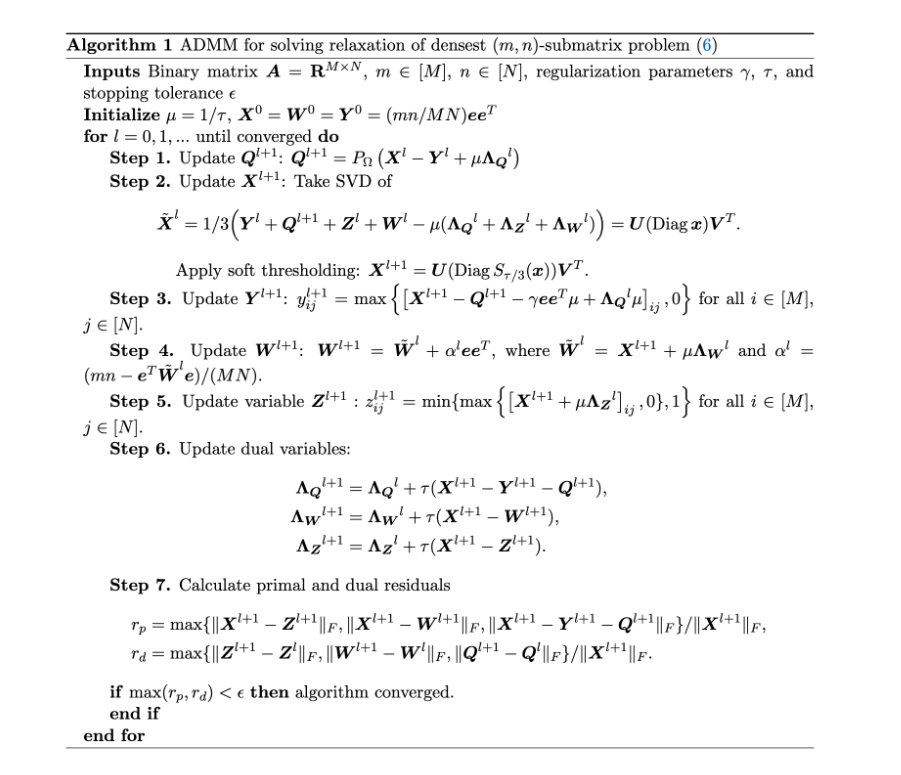
\includegraphics[width=6.25in,height=\textheight]{ALG.png}

\#Examples We test this package on differnet types of data - random
matrices sampled from the planted dense \(m \times n\) submtarix model
and real-world collaboration and communication networks.

\#\#Random matrices We generate two categories of matrices: matrix is
sparse outside the planted submatrix; noise obscuring the planted
submatrix is dense. In both the dense and sparse graphs simulations we
generate \(10\) matrices according to the planted dense submatrix model
for each choice of the parametres.

One of the examples is the famous JAZZ network that represents a
collaboration network of \(198\) musicians. Graphs consists of \(198\)
nodes and \(2742\) edges and was compiled by \textasciitilde{}.
Musicians are connected if they performed together. It is known that
this network contains a cluster of \(100\) musicians.

First we prepare the dataset for ADMM.


\end{document}
